% !TeX root = ./thesis.tex
% !TeX spellcheck = hu_HU
% !TeX encoding = UTF-8
% !TeX program = pdflatex
% !BIB program = bibtex
%TODO Change language to en_GB (recommended) or en_US for English documents
\documentclass[12pt,a4paper,oneside]{report}             % Egyoldalas (javasolt)
%\documentclass[11pt,a4paper,twoside,openright]{report}  % Duplex
\usepackage{setspace}



% thanks to http://tex.stackexchange.com/a/47579/71109
\usepackage{ifxetex}
\usepackage{ifluatex}
\newif\ifxetexorluatex % a new conditional starts as false
\ifnum 0\ifxetex 1\fi\ifluatex 1\fi>0
   \xetexorluatextrue
\fi

\ifxetexorluatex
  \usepackage{fontspec}
\else
  \usepackage[T1]{fontenc}
  \usepackage[utf8]{inputenc}
  \usepackage[lighttt]{lmodern}
\fi

\usepackage[english,magyar]{babel} % Alapértelmezés szerint utoljára definiált nyelv lesz aktív, de később külön beállítjuk az aktív nyelvet.

%\usepackage{cmap}
\usepackage{amsfonts,amsmath,amssymb} % Mathematical symbols.
%\usepackage[ruled,boxed,resetcount,linesnumbered]{algorithm2e} % For pseudocodes. % beware: this is not compatible with LuaLaTeX, see http://tex.stackexchange.com/questions/34814/lualatex-and-algorithm2e
\usepackage{booktabs} % For publication quality tables for LaTeX
\usepackage{graphicx}

%\usepackage{fancyhdr}
%\usepackage{lastpage}

\usepackage{anysize}
%\usepackage{sectsty}
\usepackage{setspace} % For setting line spacing

\usepackage[unicode]{hyperref} % For hyperlinks in the generated document.
\usepackage{xcolor}
\usepackage{listings} % For source code snippets.

\usepackage[amsmath,thmmarks]{ntheorem} % Theorem-like environments.

\usepackage[hang]{caption}

\usepackage[list=true]{subcaption}	%tof url
\usepackage{tocloft}

\usepackage{datetime2}

\singlespacing

\newcommand{\selecthungarian}{
	\selectlanguage{magyar}
	\setlength{\parindent}{2em}
	\setlength{\parskip}{0em}
	\frenchspacing
}

\newcommand{\selectenglish}{
	\selectlanguage{english}
	\setlength{\parindent}{0em}
	\setlength{\parskip}{0.5em}
	\nonfrenchspacing
	\renewcommand{\figureautorefname}{Figure}
	\renewcommand{\tableautorefname}{Table}
	\renewcommand{\partautorefname}{Part}
	\renewcommand{\chapterautorefname}{Chapter}
	\renewcommand{\sectionautorefname}{Section}
	\renewcommand{\subsectionautorefname}{Section}
	\renewcommand{\subsubsectionautorefname}{Section}
}

\usepackage[numbers]{natbib}
\usepackage{xspace}

\usepackage{url}
\usepackage{multicol} %stuff side by side

% Ide teheted a packageket amiket használni szeretnél


\makeatletter
    \setlength\@fptop{0\p@}
\makeatother


%TODO Saját adataiddal töltsd ki a kommentek szerint
%--------------------------------------------------------------------------------------
\newcommand{\szerzoVezeteknev}{Tölgyesi}
\newcommand{\szerzoKeresztnev}{Dániel}
\newcommand{\szerzoNeptun}{GHGO5W}

\newcommand{\szakirany}{\merninf{}} % automat vagy infokom

\newcommand{\konzulensAMegszolitas}{Dr.}
\newcommand{\konzulensAVezeteknev}{Kovács}
\newcommand{\konzulensAKeresztnev}{János}
\newcommand{\konzulensBMegszolitas}{}
\newcommand{\konzulensBVezeteknev}{}
\newcommand{\konzulensBKeresztnev}{}
\newcommand{\konzulensCMegszolitas}{}
\newcommand{\konzulensCVezeteknev}{}
\newcommand{\konzulensCKeresztnev}{}

\newcommand{\cim}{Okosotthonok biztonsága és sérülékenységei} % Cím
\newcommand{\tanszek}{\szeint} % automatizálási (\szeaut) vagy távközlési (\szetat)
\newcommand{\doktipus}{\szakdolgozat} % Dokumentum típusa (\szakdolgozat, \diplomaterv vagy \dolgozat)
\newcommand{\szak}{\minfBSc} % villamosmérnöki msc (\villMSc) vagy villamosmérnöki bsc (\villBSc)

%TODO Nyelv beállítása
% Beállítások magyar nyelvű dolgozathoz
%--------------------------------------------------------------------------------------
% Elnevezések
%--------------------------------------------------------------------------------------
\newcommand{\sze}{Széchenyi István Egyetem}
\newcommand{\kvik}{Gépészmérnöki, Informatikai és Villamosmérnöki Kar}
\newcommand{\szeaut}{Automatizálási Tanszék}
\newcommand{\szetat}{Távközlési Tanszék}
\newcommand{\szeint}{Informatika Tanszék}

\newcommand{\aut}{Automatizálási Szakirány}
\newcommand{\infokom}{Infokommunikáció Szakirány}
\newcommand{\merninf}{Mérnökinformatikus Szakirány}

\newcommand{\keszitette}{Készítette}
\newcommand{\konzulens}{Konzulens}

\newcommand{\szakdolgozat}{Szakdolgozat}
\newcommand{\diplomaterv}{Diplomaterv}
\newcommand{\dolgozat}{Dolgozat}

\newcommand{\villBSc}{Villamosmérnöki BSc}
\newcommand{\villMSc}{Villamosmérnöki MSc}
\newcommand{\minfBSc}{Mérnökinformatikus BSc}

\newcommand{\pelda}{Példa}
\newcommand{\definicio}{Definíció}
\newcommand{\tetel}{Tétel}

\newcommand{\bevezetes}{Bevezetés}
\newcommand{\koszonetnyilvanitas}{Köszönetnyilvánítás}
\newcommand{\fuggelek}{Függelék}

% Opcionálisan átnevezhető címek
%\addto\captionsmagyar{%
%\renewcommand{\listfigurename}{Saját ábrajegyzék cím}
%\renewcommand{\listtablename}{Saját táblázatjegyzék cím}
%\renewcommand{\bibname}{Saját irodalomjegyzék név}
%}


\newcommand{\szerzo}{\szerzoVezeteknev{} \szerzoKeresztnev}
\newcommand{\konzulensA}{\konzulensAMegszolitas\konzulensAVezeteknev{} \konzulensAKeresztnev}
\newcommand{\konzulensB}{\konzulensBMegszolitas\konzulensBVezeteknev{} \konzulensBKeresztnev}
\newcommand{\konzulensC}{\konzulensCMegszolitas\konzulensCVezeteknev{} \konzulensCKeresztnev}

\newcommand{\selectthesislanguage}{\selecthungarian}

\bibliographystyle{huplain}

\def\lstlistingname{lista}

\newcommand{\appendixnumber}{6}  % a fofejezet-szamlalo az angol ABC 6. betuje (F) lesz

% Settings for English documents
%%--------------------------------------------------------------------------------------
% Elnevezések
%--------------------------------------------------------------------------------------
\newcommand{\sze}{Széchenyi István University}
\newcommand{\kvik}{Faculty of Mechanical Engineering, Informatics and Electrical Engineering}
\newcommand{\szeaut}{Department of Automation}
\newcommand{\szetat}{Department of Telecommunications}
\newcommand{\szeint}{Department of Computer Science}

\newcommand{\aut}{Specialization in Automation}
\newcommand{\infokom}{Specialization in Infocommunication}
\newcommand{\merninf}{Specialization in Computer Science Engineering}

\newcommand{\keszitette}{Author}
\newcommand{\konzulens}{Advisor}

\newcommand{\szakdolgozat}{Bachelor's Thesis}
\newcommand{\diplomaterv}{Master's Thesis}
\newcommand{\dolgozat}{Project} % TODO not the best word for this

\newcommand{\villBSc}{Electrical Engineering BSc}
\newcommand{\villMSc}{Electrical Engineering MSc}
\newcommand{\minfBSc}{Computer Science Engineering BSc}

\newcommand{\pelda}{Example}
\newcommand{\definicio}{Definition}
\newcommand{\tetel}{Theorem}

\newcommand{\bevezetes}{Introduction}
\newcommand{\koszonetnyilvanitas}{Acknowledgements}
\newcommand{\fuggelek}{Appendix}

% Optional custom titles
%\addto\captionsenglish{%
%\renewcommand*{\listfigurename}{Your list of figures title}
%\renewcommand*{\listtablename}{Your list of tables title}
%\renewcommand*{\bibname}{Your bibliography title}
%}


\newcommand{\szerzo}{\szerzoKeresztnev{} \szerzoVezeteknev}
\newcommand{\konzulensA}{\konzulensAMegszolitas\konzulensAKeresztnev{} \konzulensAVezeteknev}
\newcommand{\konzulensB}{\konzulensBMegszolitas\konzulensBKeresztnev{} \konzulensBVezeteknev}
\newcommand{\konzulensC}{\konzulensCMegszolitas\konzulensCKeresztnev{} \konzulensCVezeteknev}

\newcommand{\selectthesislanguage}{\selectenglish}

\bibliographystyle{plainnat}

\newcommand{\ie}{i.e.\@\xspace}
\newcommand{\Ie}{I.e.\@\xspace}
\newcommand{\eg}{e.g.\@\xspace}
\newcommand{\Eg}{E.g.\@\xspace}
\newcommand{\etal}{et al.\@\xspace}
\newcommand{\etc}{etc.\@\xspace}
\newcommand{\vs}{vs.\@\xspace}
\newcommand{\viz}{viz.\@\xspace} % videlicet
\newcommand{\cf}{cf.\@\xspace} % confer
\newcommand{\Cf}{Cf.\@\xspace}
\newcommand{\wrt}{w.r.t.\@\xspace} % with respect to

\newcommand{\appendixnumber}{1}  % a fofejezet-szamlalo az angol ABC 1. betuje (A) lesz



\newcommand{\szerzoMeta}{\szerzoVezeteknev{} \szerzoKeresztnev} % egy szerző esetén TODO@FMA két szerző
%--------------------------------------------------------------------------------------
% Page layout setup
%--------------------------------------------------------------------------------------
% we need to redefine the pagestyle plain
% another possibility is to use the body of this command without \fancypagestyle
% and use \pagestyle{fancy} but in that case the special pages
% (like the ToC, the References, and the Chapter pages)remain in plane style

\pagestyle{plain}
\marginsize{35mm}{25mm}{15mm}{15mm}

\setcounter{tocdepth}{3}
%\sectionfont{\large\upshape\bfseries}
\setcounter{secnumdepth}{3}

\sloppy % Margón túllógó sorok tiltása.
\widowpenalty=10000 \clubpenalty=10000 %A fattyú- és árvasorok elkerülése
\def\hyph{-\penalty0\hskip0pt\relax} % Kötőjeles szavak elválasztásának engedélyezése


%--------------------------------------------------------------------------------------
% Setup hyperref package
%--------------------------------------------------------------------------------------
\hypersetup{
    % bookmarks=true,            % show bookmarks bar?
    unicode=true,              % non-Latin characters in Acrobat's bookmarks
    pdftitle={\cim},        % title
    pdfauthor={\szerzoMeta},    % author
    pdfsubject={\doktipus}, % subject of the document
    pdfcreator={\szerzoMeta},   % creator of the document
    pdfproducer={},    % producer of the document
    pdfkeywords={},    % list of keywords (separate then by comma)
    pdfnewwindow=true,         % links in new window
    colorlinks=true,           % false: boxed links; true: colored links
    linkcolor=black,           % color of internal links
    citecolor=black,           % color of links to bibliography
    filecolor=black,           % color of file links
    urlcolor=black             % color of external links
}


%--------------------------------------------------------------------------------------
% Set up listings
%--------------------------------------------------------------------------------------
\definecolor{lightgray}{rgb}{0.95,0.95,0.95}
\lstset{
	basicstyle=\scriptsize\ttfamily, % print whole listing small
	keywordstyle=\color{black}\bfseries, % bold black keywords
	identifierstyle=, % nothing happens
	% default behavior: comments in italic, to change use
	% commentstyle=\color{green}, % for e.g. green comments
	stringstyle=\scriptsize,
	showstringspaces=false, % no special string spaces
	aboveskip=3pt,
	belowskip=3pt,
	backgroundcolor=\color{lightgray},
	columns=flexible,
	keepspaces=true,
	escapeinside={(*@}{@*)},
	captionpos=b,
	breaklines=true,
	frame=single,
	float=!ht,
	tabsize=2,
	literate=*
		{á}{{\'a}}1	{é}{{\'e}}1	{í}{{\'i}}1	{ó}{{\'o}}1	{ö}{{\"o}}1	{ő}{{\H{o}}}1	{ú}{{\'u}}1	{ü}{{\"u}}1	{ű}{{\H{u}}}1
		{Á}{{\'A}}1	{É}{{\'E}}1	{Í}{{\'I}}1	{Ó}{{\'O}}1	{Ö}{{\"O}}1	{Ő}{{\H{O}}}1	{Ú}{{\'U}}1	{Ü}{{\"U}}1	{Ű}{{\H{U}}}1
}


%--------------------------------------------------------------------------------------
% Set up theorem-like environments
%--------------------------------------------------------------------------------------
% Using ntheorem package -- see http://www.math.washington.edu/tex-archive/macros/latex/contrib/ntheorem/ntheorem.pdf

\theoremstyle{plain}
\theoremseparator{.}
\newtheorem{example}{\pelda}

\theoremseparator{.}
%\theoremprework{\bigskip\hrule\medskip}
%\theorempostwork{\hrule\bigskip}
\theorembodyfont{\upshape}
\theoremsymbol{{\large \ensuremath{\centerdot}}}
\newtheorem{definition}{\definicio}

\theoremseparator{.}
%\theoremprework{\bigskip\hrule\medskip}
%\theorempostwork{\hrule\bigskip}
\newtheorem{theorem}{\tetel}


%--------------------------------------------------------------------------------------
% Some new commands and declarations
%--------------------------------------------------------------------------------------
\newcommand{\code}[1]{{\upshape\ttfamily\scriptsize\indent #1}}
\newcommand{\doi}[1]{DOI: \href{http://dx.doi.org/\detokenize{#1}}{\raggedright{\texttt{\detokenize{#1}}}}} % A hivatkozások közt így könnyebb DOI-t megadni.

\DeclareMathOperator*{\argmax}{arg\,max}
%\DeclareMathOperator*[1]{\floor}{arg\,max}
\DeclareMathOperator{\sign}{sgn}
\DeclareMathOperator{\rot}{rot}


%--------------------------------------------------------------------------------------
% Setup captions
%--------------------------------------------------------------------------------------
\captionsetup[figure]{
	width=.75\textwidth,
	aboveskip=10pt}

\renewcommand{\captionlabelfont}{\bf}
%\renewcommand{\captionfont}{\footnotesize\it}

%--------------------------------------------------------------------------------------
% Hyphenation exceptions
%--------------------------------------------------------------------------------------
\hyphenation{Shakes-peare Mar-seilles ár-víz-tű-rő tü-kör-fú-ró-gép}

%--------------------------------------------------------------------------------------
% Sources for figures
%--------------------------------------------------------------------------------------

% takes 3 arguments: URL, month, day
\makeatletter
\newcommand{\figsourcefont}{\footnotesize}
\newcommand{\figsource}[3]{%
  \addtocontents{lof}{%
    {\leftskip\cftfigindent
     \advance\leftskip\cftfignumwidth
     \rightskip\@tocrmarg 
     \scriptsize \url{#1} \newline Utolsó látogatás időpontja: \DTMdate{\the\year-#2-#3}
     \par}%
  }%
 }
\makeatother


\author{\szerzo}
\title{\title} % beállítások, nem kell vele foglalkoznod remélhetőleg, de ha valami latex hekkelésre vagy új parancsra van szükséged annak itt a helye


%--------------------------------------------------------------------------------------
% Itt kezdődik a dolgozat
%--------------------------------------------------------------------------------------
\begin{document}
\onehalfspacing

%TODO Feladatkiíró lap helye, csak a nyomtatott verzijóba kerül az eredeti példány
%~~~~~~~~~~~~~~~~~~~~~~~~~~~~~~~~~~~~~~~~~~~~~~~~~~~~~~~~~~~~~~~~~~~~~~~~~~~~~~~~~~~~~~
%\pagenumbering{gobble}
%--------------------------------------------------------------------------------------
% Feladatkiiras (a tanszeken atveheto, kinyomtatott valtozat)
%--------------------------------------------------------------------------------------
\clearpage
\begin{center}
\large
\textbf{FELADATKIÍRÁS}\\
\end{center}

A feladatkiíró lapot két példányban kell leadni a tanszéki adminisztrációban. Beadás előtt az egyiket visszakapod és a leadott munkába eredeti, tanszéki pecséttel ellátott és a tanszékvezető által aláírt lapot kell belefűzni (ezen oldal \emph{helyett}, ez az oldal csak útmutatás). Az elektronikusan feltöltött dolgozatban (tehát a könyvtár honlapjára feltöltött változatba) már nem kell beleszerkeszteni ezt a feladatkiírást.



\selectthesislanguage


% Címoldal
%~~~~~~~~~~~~~~~~~~~~~~~~~~~~~~~~~~~~~~~~~~~~~~~~~~~~~~~~~~~~~~~~~~~~~~~~~~~~~~~~~~~~~~
\hypersetup{pageanchor=false}
%--------------------------------------------------------------------------------------
%	The title page
%--------------------------------------------------------------------------------------
\begin{titlepage}
\begin{center}

\begin{figure}[!htb]
	\begin{minipage}{0.48\textwidth}
	  \centering
	  \hspace{-2cm}
\includegraphics[width=70mm,keepaspectratio]{figures/infologo_2020_department.png}
	\end{minipage}\hfill
	\begin{minipage}{0.48\textwidth}
	  \centering
	  \hspace{-2cm}
\includegraphics[width=70mm,keepaspectratio]{figures/infologo_2020_university.png}
	\end{minipage}
 \end{figure}
 

\vspace{120pt} %because it's the top
{\Huge \bfseries \MakeUppercase {\doktipus}}\\
\vspace{68pt}
{\huge \bfseries \cim}\\
\vspace{68pt}
{\huge \bfseries{\szerzo}}

\vspace{90pt}
\Large \textbf{\szak{}}\\
\textbf{\szakirany}\\
\vspace{90pt}
{\Large \textbf{\the\year}}

\vfill

\end{center}
\end{titlepage}
\hypersetup{pageanchor=false}



% Tartalomjegyzék
%~~~~~~~~~~~~~~~~~~~~~~~~~~~~~~~~~~~~~~~~~~~~~~~~~~~~~~~~~~~~~~~~~~~~~~~~~~~~~~~~~~~~~~
\tableofcontents\vfill
\addtocontents{toc}{\protect\thispagestyle{empty}}

% Ábrák listája - a word-ös sablon szerint szükséges
%~~~~~~~~~~~~~~~~~~~~~~~~~~~~~~~~~~~~~~~~~~~~~~~~~~~~~~~~~~~~~~~~~~~~~~~~~~~~~~~~~~~~~~
\clearpage\phantomsection
\listoffigures
\addcontentsline{toc}{chapter}{\listfigurename}

% Nyilatkozat és Kivonat
%~~~~~~~~~~~~~~~~~~~~~~~~~~~~~~~~~~~~~~~~~~~~~~~~~~~~~~~~~~~~~~~~~~~~~~~~~~~~~~~~~~~~~~
\selectlanguage{magyar}
\pagenumbering{gobble}
%--------------------------------------------------------------------------------------
% Nyilatkozat
%--------------------------------------------------------------------------------------
\begin{center}
\large
\textbf{Nyilatkozat}\\
\end{center}

\noindent
Alulírott, \textbf{\szerzoVezeteknev{} \szerzoKeresztnev{} (\szerzoNeptun)}, \szak{} szakos hallgató kijelentem, hogy a \textit{\cim} című \MakeLowercase{\doktipus{}} feladat kidolgozása a saját munkám, abban csak a megjelölt forrásokat, és a megjelölt mértékben használtam fel, az idézés szabályainak megfelelően, a hivatkozások pontos megjelölésével.

\setlength\parskip{\baselineskip}

\noindent
Eredményeim saját munkán, számításokon, kutatáson, valós méréseken alapulnak, és a legjobb tudásom szerint hitelesek.

\vspace*{24pt}
\begin{multicols}{2}
	\noindent
	Győr, \today

	\columnbreak
	\noindent
	\makebox[7cm][c]{\rule{6cm}{.4pt}}\\
	\makebox[7cm][c]{\emph{\szerzoVezeteknev{} \szerzoKeresztnev}}\\
	\makebox[7cm]{hallgató}
\end{multicols}

\thispagestyle{empty}

\vfill
\clearpage
\thispagestyle{empty} % an empty page

\selectthesislanguage
 % ez legenerálódik magától a fentebb megadott adatok alapján
\include{content/abstract} %TODO ezt át kell írnod


% A dolgozat lényegi része
%~~~~~~~~~~~~~~~~~~~~~~~~~~~~~~~~~~~~~~~~~~~~~~~~~~~~~~~~~~~~~~~~~~~~~~~~~~~~~~~~~~~~~~
\pagenumbering{arabic}

%TODO készítsd el a saját munkád
\chapter{\bevezetes}

A digitalizáció hatására ma, már minden háztartásban található vezetékes és vezeték nélküli eszköz is hozzáfér az internethez, melynek nemcsak előnye, de hátránya, hogy ezek ugyanolyan veszélynek vannak kitéve, mint bármely más, kisebb vagy nagyobb cégekhez tartozó üzleti hálózatok. Szeretném bemutatni a hálózatok működésének alapfogalmait és az okos otthoni hálózatban résztvevő eszköztípusokat, feltárom azokat a sérülékenységi lehetőségeket, melyek nagy szerepet játszanak abban, hogy eljussunk a teljesen biztonságos lakhatáshoz.
\begin{figure}[!ht]
    \centering
    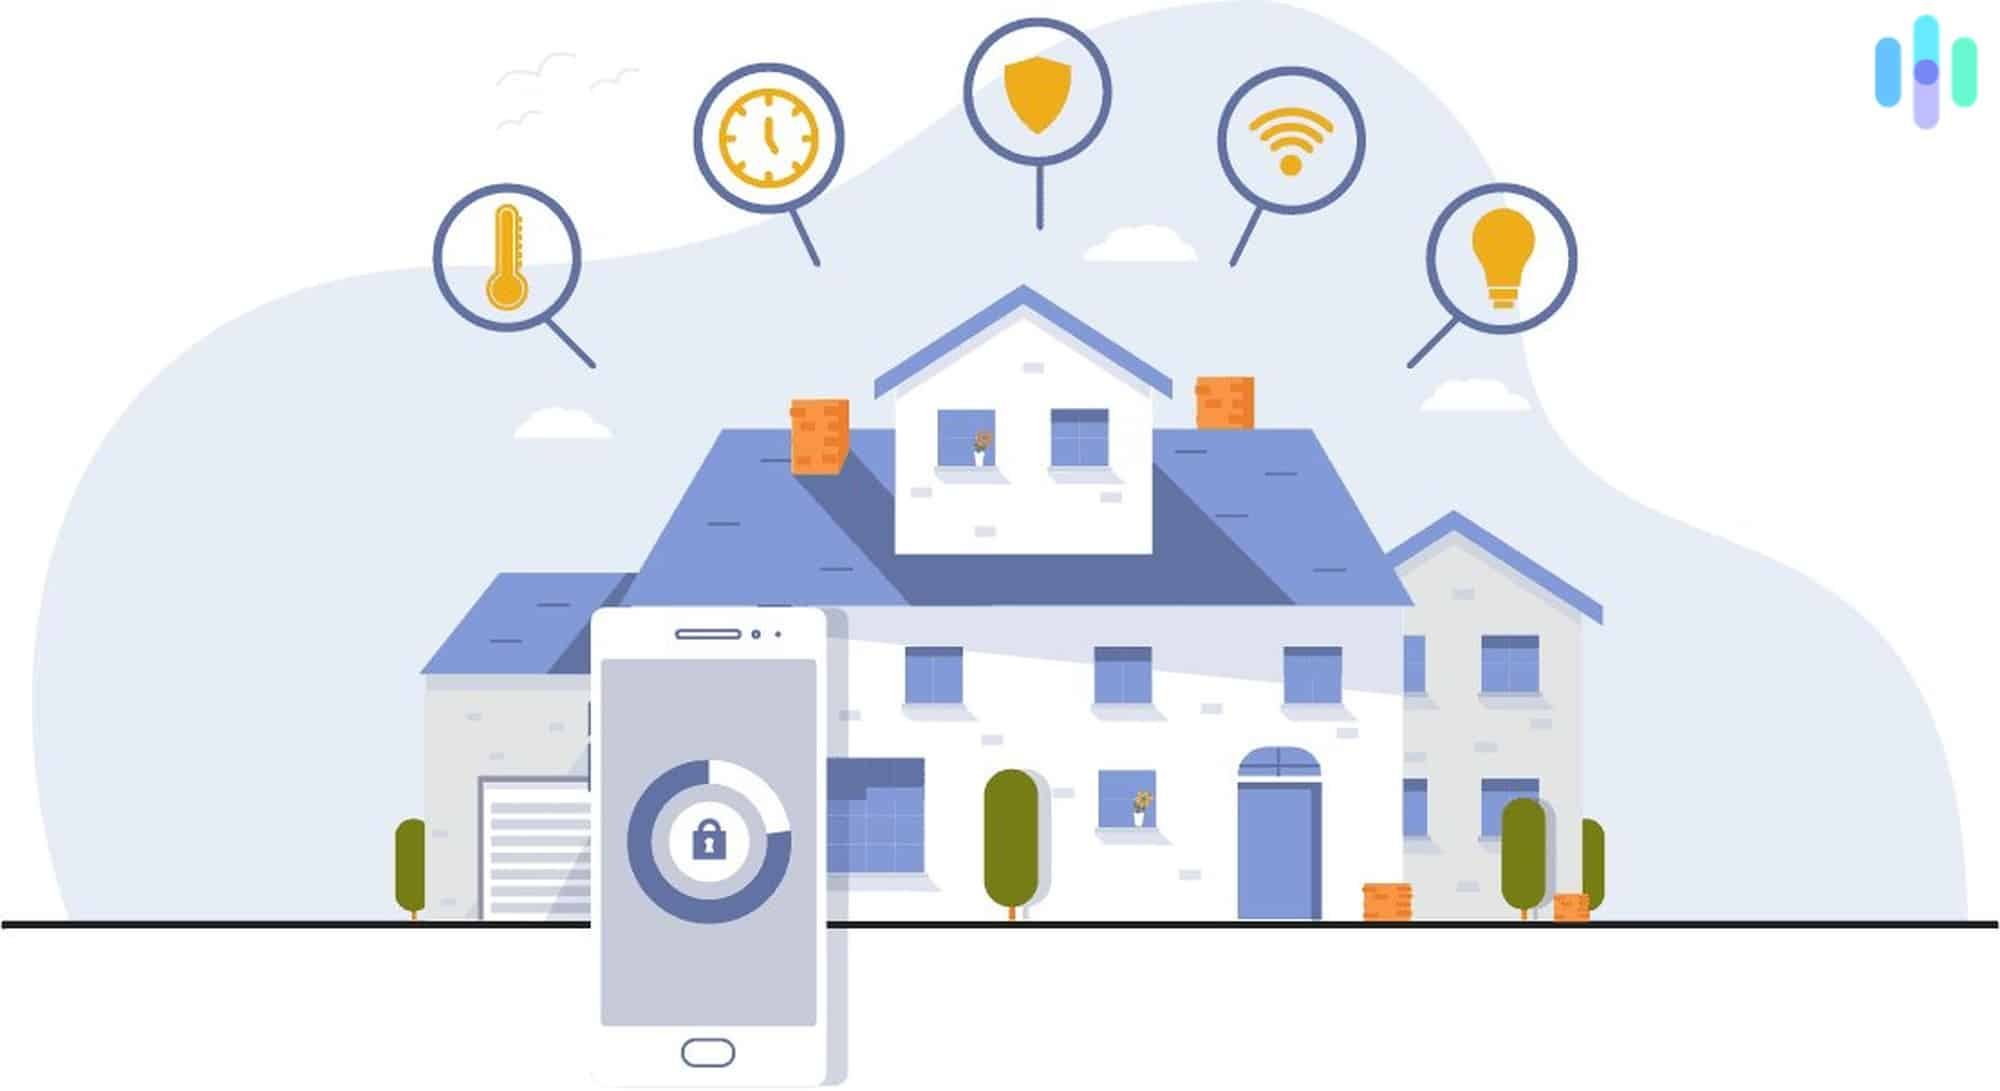
\includegraphics[width=70mm, keepaspectratio]{figures/What-is-a-Smart-Home.jpg}
    \caption{Smart home felépítése}
\end{figure}
\par Egy modern, intelligens, „okos” otthont különféle számítástechnikai és elektronikai eszközök, illetve vezeték nélküli érzékelők együttesen alkotják. Az automatizáció megjelenése során a felhasználók újabb és nagyobb elvárásokat követelnek, mely a felhasználókra szabott, fejlesztett automatizált rendszerek viselkedéséhez új utakat lehet törni. Az okosotthonok világa előtt, egy átlagos családnak közönséges betörőkkel, bűnözőkkel kellett szembe szállniuk, míg jelen pillanatban a fejlesztőknek és az okos otthonnal rendelkezőknek, számítástechnikában jártas, technikailag igencsak fejlett kiberbűnőzökkel kell felvenni a harcot, hogy megvédhessék otthonukat az esetleges külső támadásoktól. Ezek az emberek képesek megtalálni és kihasználni azokat a biztonsági réseket, amelyek alapján lehetőségük van manipulálni az adott hálózatot és az ahhoz csatlakoztatott eszközöket is, ezáltal könnyedén szabad utat nyerve a bejutáshoz. A lakatok és zárak fizikai feltörését felváltja például egy riasztórendszer tűzfalának kiiktatása vagy az automata kapunyitórendszer meg hackelése. Azonban az okosotthonok biztonsági kérdése kritikusan foglalkoztatott és fokozott figyelmet kap, viszont a technika mai állása szerint kijelenthetjük, hogy teljesen tökéletes és 100%-ig biztonságos rendszer nincsen. 
Számos kutatás és kísérletezés valósult meg az okosotthonok koncepciójával kapcsolatban az 1970-es évek vége óta. Fontos tényező, hogy mivel megfizethetőbbek és népszerűbbek lettek az elektronikus eszközök és az internethez való hozzáférés is. Hatalmas szerepet játszik az automatizálás és a kényelem, ezért egyre jobban érdeklődnek az emberek az okosotthonok iránt. 
\cite{smart-homes}
\chapter{Okosotthonok megítélése és elterjedése}

\section{Világszerte}

\section{Magyarországon}
\chapter{Alapvető definíciók ismertetése}

\section{Internet of Things}
Az IoT-ről, azaz a dolgok internetéről, akkor beszélhetünk, amikor az otthonunkban az internethez csatlakoztatott eszközök meghaladják az ott élő emberek számát. Ezeknek az eszközöknek a célja, hogy megkönnyítse mindennapi életünket, úgy, hogy egy digitális világban intelligens környezetet biztosít számunkra. intelligens eszközök segítségével adatgyűjtést végeznek a mindennapi tevékenységünkről, melyet továbbítják az úgynevezett felhőbe, hogy még precízebb képet tudjanak alkotni cselekvéseinkről. Az IoT eszközök nagyrészt vezeték nélkül csatlakoznak az internethez, mint például okos telefonok, okos otthonok és különböző az intelligens környezethez csatlakoztatható eszközök, a plug-in modulok.
\newline Az IoT 4 fő réteg szakaszból épül fel:\cite{smart-research}
\begin{itemize}
    \setlength\itemsep{-2pt}
    \item Észlelési réteg
    \item Hálózati réteg
    \item Közvetítői réteg
    \item Alkalmazási réteg 
\end{itemize}

\subsection{Smart Home}
Az intelligens otthon a technológia és a szolgáltatások integrálása az otthoni hálózatba. Rengeteg különböző technológiákat használ az otthon egyes részeinek felszerelésére az intelligensebb felügyelet és távvezérlés érdekében. A mindennapi háztartási feladatok és tevékenységek automatizálása anélkül, hogy a felhasználó beavatkozna abba.  Automatizáció implementálása a jobb életminőség érdekében. Bizonyos esetekben az otthoni szolgáltatások integrációja lehetővé teszi, hogy azok kommunikáljanak egymással az otthoni vezérlőn keresztül, ezáltal lehetővé téve, hogy egyetlen gomb segítségével különböző otthoni rendszereket vezéreljenek a mi fizikai beavatkozásunk nélkül.
\par Egy okosotthonban előre beprogramozott forgatókönyvek vagy működési módok, illetve tanulási minták alapján tervezett lépések vannak a rengeteg összegyűjtött szokási mintákból. Az intelligens otthonok javíthatják az otthoni kényelmet, komfortot, biztonságot és energiagazdálkodást. Ezen kívül az idősek és fogyatékkal élők számára is biztonságos és védett környezetet nyújthatnak.\cite{smart-home-technology}
\begin{figure}[!ht]
    \centering
    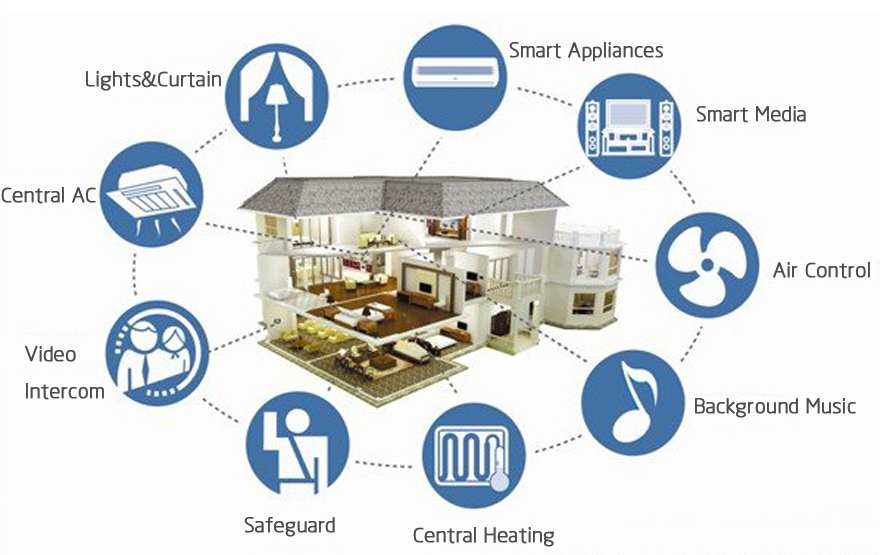
\includegraphics[width=70mm, keepaspectratio]{figures/smart-home.jpg}
    \caption{Okosotthon integrációs szolgáltatások}
\end{figure}
\par Rendkivűl pozitív előnye ennek a technológiának, hogy energiát és más erőforrásokat takarít meg. Az intelligens otthonok iránti fogyasztói lelkesedés ellenére azonban a biztonság és a védelem még mindig komoly aggodalomra ad okot. Ezek együttesen szabnak gátat a technológia elfogadásához.

\section{Biztonság}
Megállapíthatjuk, hogy a biztonság fogalma a civilizáció fejlődése során folyamatosan és exponenciálisan változik. Nehéz megfogalmazni, mivel nagyon komplex és számos területre ágaztathatjuk. Jogi biztonság, közlekedési, főként katonai és informatikai. A biztonságra való törekvés a történelem során mind az egyénben, mind a társadalomban jelen volt.
Az élet számos területein szükség van biztonsági intézkedésekre és azok elhárítására. Ma a katasztrófák vagy fenyegető vészhelyzetek olyan kihívások elé állítják a szakembereket, amelyek jellegükben, nagyságrendjükben és összetettségükben gyökeresen eltérnek a korábban tapasztaltaktól.\cite{kornyezetmernoki-tudastar} Ebben a szakdolgozatban az okosotthonok technologiájához kapcsolódó biztonsági intézkedéseket és azok sérülékenységeit fogom részletesen kifejteni és ismertetni.

\subsection{IT Security}
Ahogy a hackerek okosabbak és találékonyabbak lesznek, így még nagyobb az szükség van a digitális eszközök védelmére. Nagyrészt egy biztonságos rendszer kivitelezése költséges, de egy nem ismert biztonsági rés, jóval nagyobb pénzügyi kiesést tud okozni. A személyes adatok védelméhez informatikai biztonsági mechanizmusokra van szükség. Az IT security az információkat kezelő és tároló rendszereket, valamint az ezekbe történő feldolgozott adatokat védelmét fogalmazza meg. Az informatikai biztonságot gyakran a magánélet technikai oldalának tekintik. A biztonsági mechanizmusok belső mechanizmusok, amelyeket az informatikai rendszer valósít meg és külső mechanizmusok, amelyek a rendszeren kívül történnek. A témát öt fő részre taglalnák, amelyek közül kiemelném a hálózati biztonságot, ami lényegében megakadályozza, hogy illetéktelen felhasználók hozzáférhessenek egy hálózathoz. Ez a fajta biztonsági tényező biztosítja, hogy ne lehessen elérni az érzékeny és privát adatokat a hálózatokon keresztül.
\par Néhány szót ejtenék a végpontbiztonságról is, mely eszközszintű védelmet nyújt. A végpontbiztonság megakadályozza, hogy az eszközök hozzáférjenek a rosszindulatú hálózatokhoz, amelyek veszélyt jelenthetnek a felhasználók adataira. Naojain fejlett rosszindulatú programjaik elleni védelem és az eszközkezelő szoftverek példák a végpontbiztonságra. A végpontbiztonság által védett eszközök a táblagépek, mobiltelefonok, laptopok.
\par Tulajdonképpen minden olyan rendszerek, rendszerösszetevők, hálózati eszközök melyek alkalmasak adatok tárolására és továbbítására az IT Security fogalma alá tartoznak.\cite{cisco_2022}

\subsection{Cyber Security}
Alapesetben a kiberbiztonság a hálózatok és a rendszerek szoftveres biztonságát jelenti, számítógépekkel történő támadások ellen, viszont az elmúlt években a hálózatok a puszta kommunikációs eszközökből mindenütt jelenlévő számítástechnikai infrastrukturális hálózatokká alakultak át. A jelenlegi hálózatok nagyobbak, gyorsabbak és rendkívül dinamikusak. Ennek eredményeként a számítógépek és hálózati technológiák használata a kiberbiztonságot mára, már nemzetbiztonsági kérdéssé tette. Az internet a kormányok, vállalatok és a hétköznapi ember életének szerves része lett. A számítógépeket és a hálózatot például gyártási folyamatok kivitelezésére, tőzsdei rendszerek üzemeltetésére, légiforgalmi irányítási rendszerek kezelésére és a legújabb TikTok videó feltöltésére is használjuk. Az életünkbe való beépülés miatt a hálózati támadások elkezdték befolyásolni a valódi életünket is. Elsődleges célja egy kibertámadónak a pénzszerzés, melyet többféle módon is kivitelezhet. Célpont lehet közvetlenül egy kiszemelt bank, ami lássuk be nehezebben megvalósítható, viszont könnyebb préda egy ártatlan bankkártyafelhasználó. Különféle módok vannak a felhasználói adatok megszerzésére, amihez kizárólag a bankfiók tulajdonosát kell „meghackelni”, ezt nevezzük a Social Engineeringnek. Ebben az esetben az ember a kulcs és a gyenge láncszem. A felhasználóknak meg kell érteniük és be kellene tartaniuk olyan alapvető szabályokat és biztonsági előírásokat, mellyel megelőzhető lenne a személyes adataiknak a kiszivárgása. 
\par A digitális világban végrehajtott bűncselekményeket 3 fő csoportra oszthatjuk fel, ezek közül az elsőként említendő és a köztudatban a legelterjedtebb a kiberbűnözés, amely véghezvihető egyedül és csoportban is. Ezek a támadások legfőképpen pénzszerzés céljából alakulnak ki, a rendszer vagy hálózat sérülékenységeit kihasználva nyerészkednek, vagy kárt tesznek abban. 
\begin{figure}[!ht]
    \centering
    
\includegraphics[width=70mm, keepaspectratio]{figures/274638343_482850443543049_4683554889010609984_n.jpg}
    \caption{Anonymous hackercsoport szimbóluma}
\end{figure}
\par A kiberterror, az a jelenség, amikor a digitális világ adta előnyöket kihasználva információs infrastruktúrákat támadnak vagy ezen keresztül félemlítenek meg embereket, előre megfontolva ugyanúgy egyedül vagy csoportosan.
\par Az utolsó ismertetett fogalom a kiber támadás, amelynek általában a legfőbb célpontjai nagyobb csoportok, mint például egy ország vagy nemzet.\cite{cybersecurity}


\include{content/okosotthon-bemutatása.tex}
\chapter{Okosotthon előnyei és hátrányai}
\chapter{Az okosotthonok elleni kibertámadások}

\section{Bűnözők a monitor másikfelén}
\section{Script kiddies}


\section{Elterjedt ámadási technikák}

\subsection{Támadások egyik}
\subsubsection{Phising websites}




\subsection{Támadások másik}


\section{Biztonsági sérülékenységek a hálózaton}

\section{Kibertámádások elhárítása}
\subsection{}


%\include{content/analizalas}
%\include{content/introduction}
%\include{content/thesis-format}
%\include{content/latex-tools}
%\include{content/template-usage}


% Köszönetnyilvánítás - opcionális
%~~~~~~~~~~~~~~~~~~~~~~~~~~~~~~~~~~~~~~~~~~~~~~~~~~~~~~~~~~~~~~~~~~~~~~~~~~~~~~~~~~~~~~
%\include{content/acknowledgement}


% Táblázatok listája - opcionális
%~~~~~~~~~~~~~~~~~~~~~~~~~~~~~~~~~~~~~~~~~~~~~~~~~~~~~~~~~~~~~~~~~~~~~~~~~~~~~~~~~~~~~~
%\clearpage\phantomsection
%\listoftables
%\addcontentsline{toc}{chapter}{\listtablename}


% Irodalomjegyzék
%~~~~~~~~~~~~~~~~~~~~~~~~~~~~~~~~~~~~~~~~~~~~~~~~~~~~~~~~~~~~~~~~~~~~~~~~~~~~~~~~~~~~~~
\clearpage\phantomsection
\bibliography{bib/mybib}
\addcontentsline{toc}{chapter}{\bibname}


% Függelékek
%~~~~~~~~~~~~~~~~~~~~~~~~~~~~~~~~~~~~~~~~~~~~~~~~~~~~~~~~~~~~~~~~~~~~~~~~~~~~~~~~~~~~~~
%\include{content/appendices}

%\label{page:last}
\end{document}
